%Siehe tolle Daten in Tab. \ref{tab:impl:data}.
%
%%\begin{table}
%%    \centering
%%    \begin{tabular}{|lcc|}
%%    \hline
%%              & \textbf{Regular Customers} & \textbf{Random Customers} \\ \hline
%%    Age       & 20-40                      & \textgreater{}60          \\ \hline
%%    Education & university                 & high school               \\ \hline
%%    \end{tabular}
%%    \caption{Ein paar tabellarische Daten}
%%    \label{tab:impl:data}
%%\end{table}
%%
%%\begin{figure}
%%    \centering
%%    
\includegraphics[scale=0.5]{pics/knuthi.jpg}
%%    \caption{Don Knuth -- CS Allfather}
%%    \label{fig:impl:knuth}
%%\end{figure}
%%
%%Siehe und staune in Abb. \ref{fig:impl:knuth}.
%%\lipsum[6-9]
%%Dann betrachte den Code in Listing \ref{lst:impl:foo}.
%%
%%\begin{lstlisting}[language=Python,caption=Some code,label=lst:impl:foo]
%%# Program to find the sum of all numbers stored in a list (the not-Pythonic-way)
%%
%%# List of numbers
%%numbers = [6, 5, 3, 8, 4, 2, 5, 4, 11]
%%
%%# variable to store the sum
%%sum = 0
%%
%%# iterate over the list
%%for val in numbers:
%%    sum = sum+val
%%
%%print("The sum is", sum)
%\end{lstlisting}

\section{Aufbau}\label{sec:assembly}

Folgend werden alle Gegenstände und Geräte für den Aufbau in Abbildung~\ref{fig:assembly} benannt.

\begin{figure}
    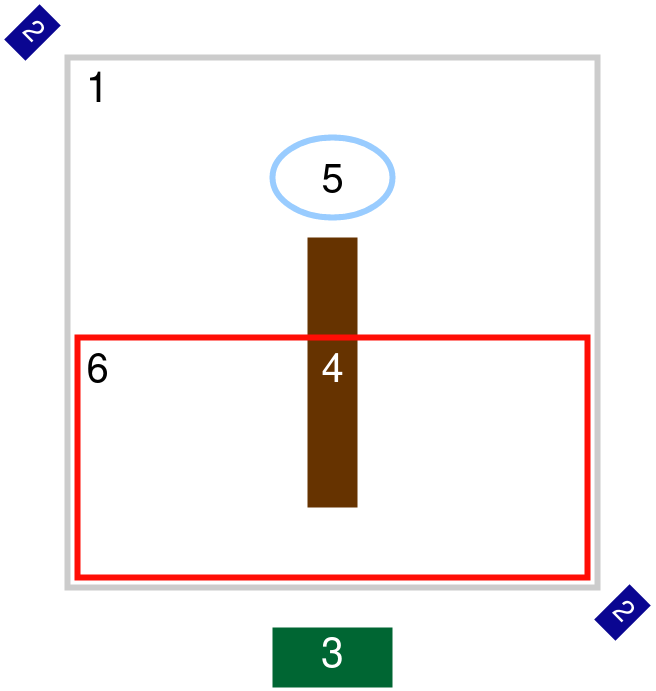
\includegraphics[scale=0.5]{pics/assemlbly}
    \caption{Aufbau}
    \label{fig:assembly}
\end{figure}

\begin{enumerate}
    \item VR Raum
    \item Lichtboxen~\ref{sec:lighthouse}
    \item Bildschirm
    \item Balken
    \item Startposition
    \item Abgrund
\end{enumerate}

\subsection{Erklärung}\label{subsec:description}

Der Spieler bei der Startposition starten und dann Richtung Abgrund dem Balken entlang balancieren.
Die Lichtboxen müssen diagonal positioniert werden wie bereits beschrieben in dem Abschnitt~\ref{sec:lighthouse}.
Der Balken sollte ca in der Mitte sein.

Leichte Versetzungen sidn nicht tragisch. Hierbei geht es nur darum, dass der Balken nicht aus dem VR Raum
rausschaut, da das Tracking dort abbricht. Die position des Bildschirmes ist nicht wichtig.
Hierbei geht es nur um das Steam VR Setup welches bereits in dem Kapitel Steam besprochen worden ist.

\section{Code}\label{sec:code}
\subsection{Ganzkörper-Tracking}\label{sec:full-body-tracking}
\subsection{Beam Calibration}\label{subsec:beam-calibration}
\subsection{Schwerkraft}\label{subsec:gravity}
\subsection{Verkehrssystem}\label{subsec:traffic-system}
\section{3d Welt}\label{sec:3d-world}
\subsection{City Grid System}\label{subsec:city-grid-system}
\subsection{Stadt}\label{subsec:city}
\subsection{Tag Stadt}\label{subsec:day-city}
\subsection{Nacht Stadt}\label{subsec:night-city}
\subsection{Apokalypsen Stadt}\label{subsec:apocalypse-city}
\section{Sound Design}\label{sec:sound}
\subsection{Apocalypse}\label{subsec:apocalypse-background-sound}
\subsection{City}\label{subsec:day-night-background-sound}
\subsection{Event}\label{subsec:building-collapse-sound}
\section{Effects}\label{sec:effects}
\subsection{Nebel}\label{subsec:fog-effect}
\subsection{Lichter}\label{subsec:light-effect}
\subsection{Wind}\label{subsec:wind-effect}
\section{Unity Prefabs}\label{sec:prefabs}
\subsection{Game}\label{subsec:game-prefab}
\subsection{CameraRigGame}\label{subsec:camera-rig-game-prefab}
\subsection{CameraRigMenu}\label{subsec:camera-rig-menu-prefab}
\section{Inbetriebnahme}\label{sec:commissioning}
